\documentclass[]{article}

\usepackage{hyperref}
\usepackage{microtype}
\usepackage{float}
\usepackage{graphicx}

\title{\texttt{23\_14} Web Scraper}
\author{boa (\texttt{boaboa})}

\begin{document}

\maketitle

\begin{abstract}

%Write a program that extracts and aggregates news headlines from various sources.
%With Copilot, you can get help on understanding various web scraping techniques and libraries.



\end{abstract}

\pagebreak

\section{Tervezés}

A ChatGPT promptolásánál mindig angol nyelvű szöveget használtam, mert abban jobb a modell (lévén, hogy tanítás abból közben többet látott).

\begin{figure}[H]
	\centering
	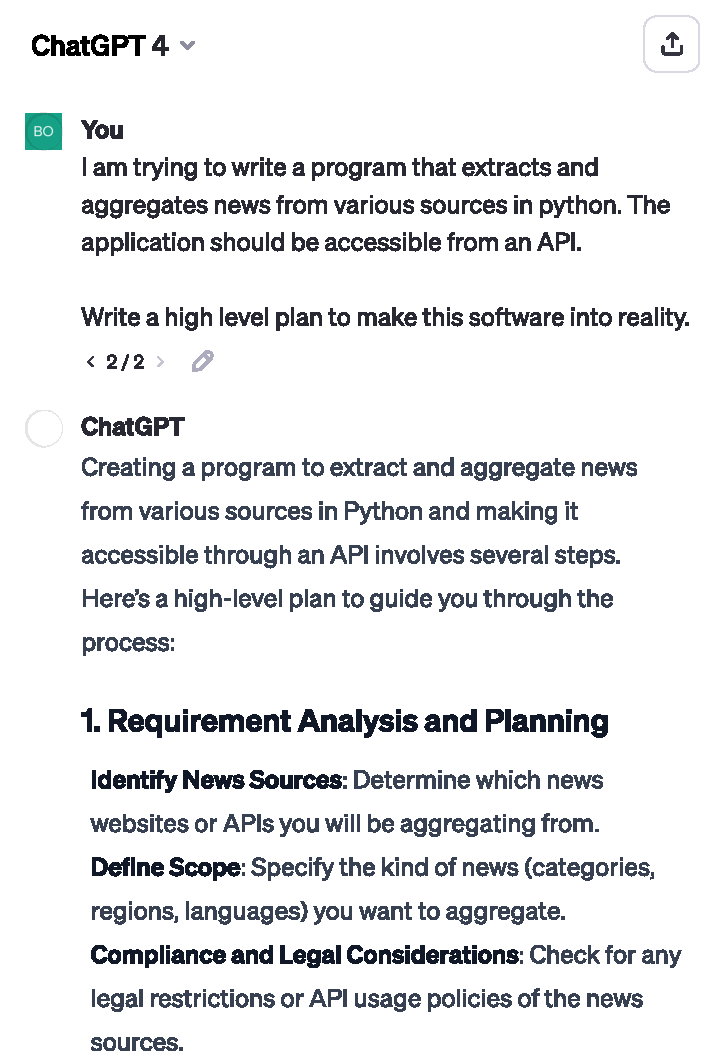
\includegraphics[width=0.7\textwidth]{prompt_1.pdf}
	\caption{Kezdeti prompt (nem teljes válasz)}
\end{figure}

A ChatGPT kimenetét megvizsgálva és saját tudásomra támaszkodva úgy döntöttem RSS folyamok periódikus letöltésével fogom az új híreket megszerezni. A teljes szöveghez viszont általában csak az cikket tartalmazó oldal letoltése és értelmezése után lehet hozzáférni, erre \texttt{Beautiful Soup} Python könyvtárat választottam. Az adatok eltárolását az egyszerűség kedvéért egy lokális Sqlite adatbázissal oldottam meg. Végül pedig az adatokat \texttt{FastApi} python könyvtár segítségével tettem elérhetővé egy API endpointon.

\section{Megoldás}

\subsection{Alapok}

\begin{figure}[H]
	\centering
	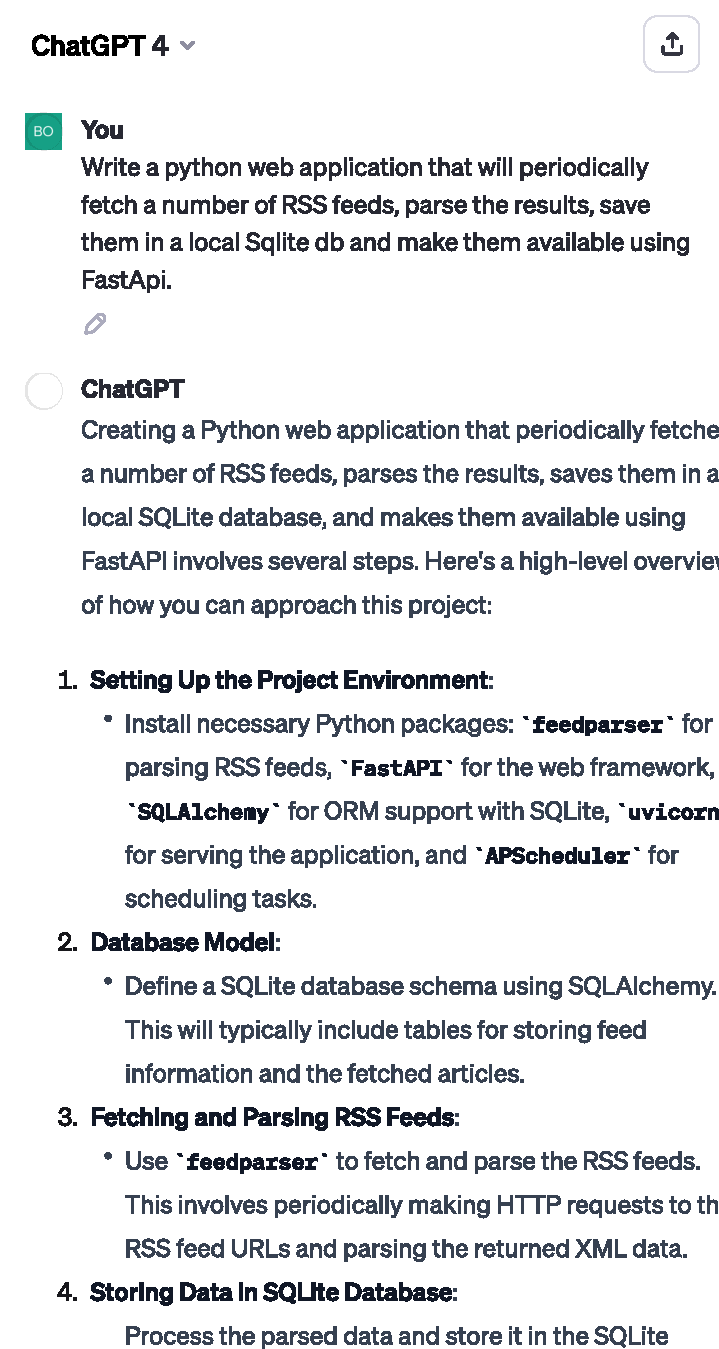
\includegraphics[width=0.65\textwidth]{prompt_2.pdf}
	\caption{Impelementációhoz prompt (nem teljes válasz)}{Ez a prompt persze nem produkált elsőre tökéletesen műdödő szoftvert, bőven volt mit kiegészíteni.}
\end{figure}

Az elkészült projekt \texttt{feedparser}-t alkalmaz az RSS feed-ek elemzéséhez, \texttt{FastAPI}-t a webes keretrendszerhez, \texttt{SQLAlchemy}-t az ORM támogatáshoz SQLite-al, \texttt{uvicorn}-t az alkalmazás szolgáltatásához, és \texttt{APScheduler}-t az időzített feladatokhoz.

A szoftver ki lett egészítve egy funkcióval a duplikált cikkek kezelésére, amely magában foglalja az egyedi cím és link kombinációk ellenőrzését az adatbázisban, mielőtt azokat hozzáadná. A \texttt{feedparser} által visszaadott \texttt{published\_parsed} dátumokat \texttt{datetime} objektummá alakítottuk, hogy kompatibilisek legyenek az SQLite \texttt{DateTime} típusával.

A programot továbá úgy módosítottam, hogy az rss feedek listáját egy json fájlból olvassa be.

\subsection{Részletesebb adatok parsolása}

Az eddigi megoldást még ki akartam egészíteni azzal, hogy a cikkek teljes szövegét letöltöm, ami alapból nem szokott az RSS folyamban eltárolva lenni.

\section{Verziókövetés}

A megoldás és a dokumentáció forráskódja a következő git repository-ban elérhető: \url{https://github.com/boapps/hu-news-scraper}



\end{document}
